% LaTeX Article Template - customizing header and footer
\documentclass{article}

\newtheorem{thm}{Theorem}

% Set left margin - The default is 1 inch, so the following 
% command sets a 1.25-inch left margin.
\setlength{\oddsidemargin}{0.25in}

% Set width of the text - What is left will be the right margin.
% In this case, right margin is 8.5in - 1.25in - 6in = 1.25in.
\setlength{\textwidth}{6in}

% Set top margin - The default is 1 inch, so the following 
% command sets a 0.75-inch top margin.
\setlength{\topmargin}{-0.25in}

% Set height of the header
\setlength{\headheight}{0.3in}

% Set vertical distance between the header and the text
\setlength{\headsep}{0.2in}

% Set height of the text
\setlength{\textheight}{9in}

% Set vertical distance between the text and the
% bottom of footer
\setlength{\footskip}{0.1in}

% Set the beginning of a LaTeX document
\usepackage{tikz}
\usepackage{multirow}
\usepackage{fullpage}
\usepackage{graphicx}
\usepackage{amsthm}
\usepackage{url}
\usepackage{amssymb}
\usepackage{amssymb}
\usepackage{algpseudocode}
\graphicspath{%
    {converted_graphics/}% inserted by PCTeX
    {/}% inserted by PCTeX
}
%%%%%%%%%%%%%%%%%%%%%%%%%%%%%




\begin{document}\title{Homework $2$\\ Computer Science \\ B551 Spring 2018\\ Hasan Kurban}         % Enter your title between curly braces
\author{Jinju Jiang(Hellen)}        % Enter your name between curly braces
\date{\today}          % Enter your date or \today between curly braces
\maketitle


% Redefine "plain" pagestyle
\makeatother     % `@' is restored as a "non-letter" character




% Set to use the "plain" pagestyle
\pagestyle{plain}
\section*{Introduction}
The aim of this homework is to get you acquianted with problem solving and the steps  (Real World $\rightarrow$ Concept $\rightarrow$ Logic  $\rightarrow$ Implementation).  You will turn-in four files\begin{itemize} \item A *pdf with the written answers called \texttt{hw2.pdf} \item A Python script called \texttt{rv1.py} \item  A Python script called  \texttt{rv2.py} \item A Python script called \texttt{rpsg.py}  for rock-paper-scissors.\end{itemize}  I am providing this \LaTeX{} document for you to freely use as well. Please enjoy this homework and ask yourself what interests you and then how can you add that interest to it!  Finally, questions 4 and 5 are
worth 50 points each whereas questions 1,2 and 3 are 20 worth points each.

\newpage
\section*{Homework Questions}
\begin{enumerate}
\item Problem 3.10 (p. 115) in the text.
\item Problem 3.18 (p. 117) in the text.
\item The text (page 95) describes consistency as:
\begin{eqnarray*}
h(n) &\leq c(n,a,n') + h(n')
\end{eqnarray*}
for state $n$, its successor $n'$ and action $a$.  For $G = (\{A,B,C\},\{(A,B), (A,C), (B,C)\})$, $Cost = \{((A,B),2), ((A,C),5), ((B,C), 1)\}$, and $h(A) = 1, h(B) = 4, h(C) = 3$. Is this consistent?
  

\item Assume you're programming a robot named \textsf{R} to navigate a 2D surface.  The robot can only move forward a single step to an adjacent square (not diagonally), but can also rotate $\pm$ 90 degrees.  \textsf{R} has a single sensor on its front that determines if there is an obstruction, perhaps a wall, is in its path.  Your task is to read in a 2D plan and starting at location from the southmost (bottom) side, navigate to another side.  The plan below has an opening at (3,1).  {\it One} path is: (3,1), (3,2), $\ldots$, (3,5), (2,5), (1,5).  If \textsf{R} is at (4,2) facing north, then its sensor would return 1.  If \textsf{R} is at (4,2) and facing east, its sensor would return 0.  If \textsf{R} is at (2,2) facing west, to move to (3,2), rotate(90), rotate(90), step.  You can {\it start} \textsf{R} on any available open square on the bottom -- you'll have to decide what direction \textsf{R} is facing.  The plan is encoded as an array of ones and zeros.  The plan below:

\begin{center}
{\small
\begin{tikzpicture}
\draw[step=1cm,black,thin] (0,0) grid (6,6);
\draw[fill=blue](1,0) rectangle (2,1);
\draw[fill=blue](3,2) rectangle (4,3);
\draw[fill=blue](3,0) rectangle (4,1);
\draw[fill=blue](4,0) rectangle (5,1);
\draw[fill=blue](5,0) rectangle (6,1);
\draw[fill=blue](5,1) rectangle (6,2);
\draw[fill=blue](5,2) rectangle (6,3);
\draw[fill=blue](5,3) rectangle (6,4);
\draw[fill=blue](5,4) rectangle (6,5);
\draw[fill=blue](5,5) rectangle (6,6);
\draw[fill=blue](0,1) rectangle (1,2);
\draw[fill=blue](0,0) rectangle (1,1);
\draw[fill=blue](1,5) rectangle (2,6);
\draw[fill=blue](2,2) rectangle (3,3);
\draw[fill=blue](2,5) rectangle (3,6);
\draw[fill=blue](3,5) rectangle (4,6);
\draw[fill=blue](4,5) rectangle (5,6);
\draw[fill=blue](3,4) rectangle (4,5);
\draw[fill=blue](0,2) rectangle (1,3);
\draw[fill=blue](0,3) rectangle (1,4);
\draw[fill=blue](0,5) rectangle (1,6);
\draw[fill=blue](1,2) rectangle (2,3);
\end{tikzpicture}}
\end{center}

would be encoded as:

\begin{verbatim}
111111
000100
100001
111101
100001
110111
\end{verbatim}
\begin{enumerate}
\item Given a floor plan \texttt{f.txt} (read in the file),  return \textsf{True} and the series of instructions needed to navigate \textsf{R} if there is a path and \textsf{False} otherwise.  Name this program \texttt{rv1.py}.
\item Improve \textsf{R}'s programming by returning the {\it shortest} path if it exists.  Name this program \texttt{rv2.py}.
\item Discuss your search techniques in both solutions.   State explicitly your $\hat{h}, \hat{g}, \hat{f}$.
\end{enumerate}
\item Extend Rock/Paper/Scissors from the last assignment that has the computer playing a human. You'll additionally have \$100 dollars worth of \$1 chips.  {\it Before} you show your selection, you must place a wager (at least \$1).  Keep the computer's strategy uniform and independent for both how it plays and how it bets.  The maximum amount of chips that can be wagered is $\mathrm{min}\{c,h\}$ where $c,h$ are the counts of computer and human chips respectively.  Compare this R/P/S with your earlier version and discuss.  Name this program \texttt{rpsg.py}.  

\end{enumerate}
\end{document}
